\documentclass{standalone}
\usepackage{tikz}
\usepackage{ctex,siunitx,ninecolors}
\setCJKmainfont{Noto Serif CJK SC}
\usepackage{tkz-euclide}
\usepackage{amsmath}
\usepackage{wasysym}
\usetikzlibrary{patterns, calc}
\usetikzlibrary {decorations.pathmorphing, decorations.pathreplacing, decorations.shapes,}
\begin{document}
\small
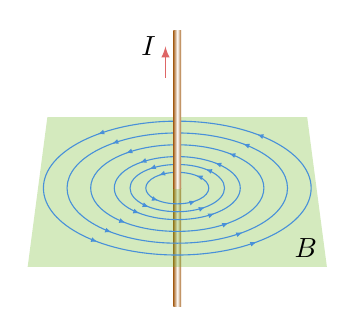
\begin{tikzpicture}[>=latex,scale=1]
  \fill[left color=brown5,right color =brown5,middle color=white](-0.05,-1.5)rectangle(0.05,0);
  \fill [olive7,opacity=0.3](1.9,-1)--(1.65,0.9)--(-1.65,0.9)--(-1.9,-1);
  \foreach \ra/\rb in { 0.4/0.2, 0.6/0.3 ,0.8/0.4, 1.1/0.55,1.4/0.7,1.7/0.85}
  {
  \draw[postaction={decorate},decoration={markings,mark={between positions 0.125 and 0.875 step 0.25 with {\arrow{Latex[scale=0.5]}}}},azure6]
    (0,0) ellipse [x radius=\ra cm, y radius=\rb cm];
  } 
  \fill[left color=brown5,right color =brown5,middle color=white](-0.05,0)rectangle(0.05,2);
  \draw[->,red6](-0.15,1.4)--(-0.15,1.8)node[left,text=black]{$I$};
  \node at (1.9,-1)[above left,text=black]{$B$};
\end{tikzpicture}
\end{document}